\chapter{Thermodynamique (spé)}

\newpage

\section{Premier principe sur un fluide en écoulement stationnaire $\bullet\circ\circ\circ$}

Préciser les hypothèses et établir l'expression générale du premier principe pour un fluide en écoulement stationnaire à travers une machine quelconque sous la forme (les grandeurs thermodynamiques massiques sont en minuscule) :
\begin{align*}
	\Delta (h+e_p+e_c)=w_u+q
\end{align*}
Préciser la signification physique de chacun des termes et son unité.
Même question, en faisant apparaître le débit massique du fluide $D_m$ :
\begin{align*}
	D_m\Delta (h+e_p+e_c)=P_u+P_{th}
\end{align*}

\newpage

\section{Second principe sur un fluide en écoulement stationnaire $\bullet\circ\circ\circ$}

Préciser les hypothèses et établir l'expression générale du second principe pour un fluide en écoulement stationnaire à travers une machine quelconque sous la forme (les grandeurs thermodynamiques massiques sont en minuscule) :
\begin{align*}
	\Delta s=s_{ech}+s_{créée}
\end{align*}
Préciser la signification physique de chacun des termes et son unité.
Même question, en faisant apparaître le débit massique du fluide $D_m$ :
\begin{align*}
	D_m\Delta s=\dot{S}_{ech}+\dot{S}_{créée}
\end{align*}

\newpage

\section{Pompe de relevage $\bullet\circ\circ\circ$}

Une pompe de relevage est une machine remontant un fluide de masse volumique $\rho$ d'un dénivelé $h$. On supposera que les sections d'entrée et de sortie du fluide sont identiques. 

\begin{enumerate}

	\item Préciser les hypothèses et établir l'expression générale du premier principe pour un fluide en écoulement stationnaire à travers une machine quelconque sous la forme (les grandeurs thermodynamiques massiques sont en minuscule) :
\begin{align*}
	\Delta (h+e_p+e_c)=w_u+q
\end{align*}
Préciser la signification physique de chacun des termes et son unité.
	\item Même question, en faisant apparaître le débit massique du fluide $D_m$ :
\begin{align*}
	D_m\Delta (h+e_p+e_c)=P_u+P_{th}
\end{align*}
	
	\item Lors du passage dans la machine, y a t-il variation d'énergie cinétique, potentielle ou thermique ?
	
	\item Exprimer la puissance de la pompe $p$ pour relever le fluide avec un débit massique $d$. 
	
	\item Rappeler les densités typiques d'un gaz et d'un liquide. Ce type de machine est-il couramment utilisé pour relever des gaz ou des liquides ?

\end{enumerate}

\newpage

\begin{correction}

\begin{enumerate}

	\item Il n'y a uniquement que de la variation d'énergie potentielle ; les sections d'entrée et de sortie étant identiques, il n'y a pas de variation d'énergie cinétique ; une pompe ne chauffe pas, donc pas de variation de température.
	
	\item On applique le premier principe industriel :
	\begin{align*}
		dgh = p
	\end{align*}
	
	\item Densité d'une phase condensée : $\rho\simeq1-8\times10^3$kg/m$^3$, d'un gaz : $\rho\simeq1\times$kg/m$^3$. On l'utilise pour les liquides.

\end{enumerate}

\end{correction}

\newpage

\section{Ecoulement d'un torrent}

Un torrent s'écoule sur une montagne sur un dénivelé de 1000m, du fait de sa viscosité et des turbulences, la vitesse reste constante lors de son trajet. Pour simplifier, on suppose que l'écoulement est adiabatique car suffisament rapide pour pouvoir négliger les tranferts thermiques. 

\begin{enumerate}

\item

\begin{enumerate}

	\item Calculer l'échauffement de l'eau lors de sa descente. La capacité calorifique de l'eau est $c_P=4$kJ/K/kg. 
	
\end{enumerate}

\item On souhaite comparer de ce qui, entre l'air et l'eau, s'échauffe le plus lors de la descente en montagne. On suppose aussi qu'un écoulement d'air decend sur le même dénivelé de manière adiabatique et réversible. 

\begin{enumerate}

	\item Montrer que la variation d'enthalpie massique de l'air peut s'écrire :
	\begin{align*}
		\Delta h =\frac{\gamma R}{M(\gamma -1)}\Delta T
	\end{align*}
	où $M=29$g/mol est la masse molaire de l'air.

	\item Comparer avec la différence de température de l'air entre le haut et le bas de la montagne. Qui s'échauffe le plus entre l'eau et l'air ?
	
	\item Quelle est la variation d'entropie massique de cet écoulement d'air ? 
	
\end{enumerate}

\end{enumerate}

\newpage

\begin{correction}

\begin{enumerate}

\item On applique le premier principe industriel : $c_p\Delta T+g\Delta z=0$. On trouve que $\Delta T = 0,25$ K, ce qui est très faible : l'eau ne s'échaufe que très peu.

\item On rappelle que la variation d'entropie de $n$ moles de gaz s'écrit $\Delta H=\frac{nR\gamma}{\gamma-1}\Delta T$

\end{enumerate}

\end{correction}

\newpage

\section{Compresseur}

Un compresseur augmente la pression d'un gaz parfait arrivant au débit massique $d_m$ de $P_1$ à $P_2$, on notera $a=P_2/P_1$ le taux de compression. La section dans laquelle circule le gaz est supposé constante. On suppose dans un premier temps que la compression est adiabatique et réversible.

\begin{enumerate}

\item

\begin{enumerate}

	\item Citer deux exemples d'objet utilisant un compresseur à flux continu.
	
	\item Quelle est la température $T_2$ du gaz en sortie du compresseur ?
	
	\item En déduire le travail massique $w_u$ nécessaire pour comprimer ce gaz. Exprimer aussi la puissance $p_u$ de ce compresseur.

\end{enumerate}

\item

On suppose désormais que les pertes thermiques sont importantes : la compression n'est plus adiabatique, elle est isotherme. 

\begin{enumerate}

	\item Quelle est le travail massique $w_u$ nécessaire pour comprimer ce gaz dans ce cas-là ? En déduire la chaleur massique $q$ perdue par le gaz. 
	
	\item Calculer la variation d'entropie massique $\Delta s$ du gaz lors de la compression.
	
\end{enumerate}

\end{enumerate}

\newpage

\section{Tuyère}

Une tuyère est un dispositif utilisé dans l'aérospatiale, dans laquelle un gaz chaud issu d'une combustion est accéléré en se refroidissant : elle convertit l'énergie thermique du gaz en énergie cinétique, servant à la propulsion d'un engin. Une tuyère (représentée ci-dessous, avec un profil divergent $(1)$ et un profil convergent $(2)$) est un conduit de symétrie de révolution selon l'axe $Ox$, de section variable ($S(x)$ à l'abscisse $x$), dont les parois sont calorifugées, sans aucune pièce mécanique à l'intérieur.

\begin{figure}[!h]
\centering
	
\includegraphics[width=0.9\linewidth]{thermo_tuyere.pdf}
\end{figure}

Les gaz issus de la combustion, de capacité calorifique $c_P$, sont, en $x=0$, à la température $T_0$ et à la vitesse $v_0$. On note $T(x)$ et $v(x)$ la température et la vitesse du gaz à l'abscisse $x$. On formule les hypothèses suivantes :
\begin{itemize}
	\item Le gaz est très chaud à l'entrée de la tuyère et sa vitesse faible, c'est-à-dire que $\frac{1}{2}v_0^2\ll c_PT_0$ ; 
	\item La section $S(x)$ varie lentement de sorte que la vitesse du gaz est orthogonale en tout point de la section $S(x)$ ;
	\item La vitesse du gaz est toujours inférieure à celle du son.
\end{itemize}

\vspace{1cm}

A partir de ces hypothèses, la tuyère doit-elle avoir un profil divergent $(1)$ ou convergent $(2)$ pour que les gaz soient accélérés ?

\newpage

\begin{correction}

Il faut déterminer la température et la vitesse dans la tuyère. Le premier principe industriel s'écrit :
\begin{align*}
	\frac{1}{2}v^2(x)+c_PT(x)=\frac{1}{2}v^2_0+c_PT_0
\end{align*}
Pour obtenir une nouvelle équation sur $T$, on peut utiliser la loi de Laplace, qui s'écrit :
\begin{align*}
T(x)\rho(x)^{1-\gamma}=T_0\rho_0^{1-\gamma}
\end{align*}
où $\rho$ est la masse volumique du gaz. Avec la conservation du débit massique, on obtient une dernière équation :
\begin{align*}
	D_m=\rho(x)v(x)S(x)=\rho_0v_0S_0
\end{align*}
En injectant dans l'équation du premier principe, on obtient :
\begin{align*}
	\frac{1}{2}v^2(x)+c_PT_0\left( \frac{v(x)S(x)}{v_0S_0}\right)^{1-\gamma}=\frac{1}{2}v^2_0+c_PT_0
\end{align*}
On introduit la quantité $u(x)=v(x)/v_0$, $\sigma(x)=S(x)/S_0$ et $\eta_0=2c_PT_0/v_0^2$. D'après les hypothèses de l'énoncé, $\eta_0\ll1$. Alors :
\begin{align*}
	u^{\gamma+1}(x)+\eta_0\sigma^{1-\gamma}(x)=(1+\eta_0)u^{\gamma-1}(x)
\end{align*}
On a donc une équation permettant de connaitre directement la vitesse en fonction de la section, même s'il faut tout de même un petit coup de main numérique pour avoir le profil exact. Néanmoins, on peut ruser pour savoir s'il faut un profil divergent ou convergent, en dérivant cette équation :
\begin{align*}
	(\gamma+1)u'(x)u^{\gamma}(x)+(1-\gamma)\eta_0\sigma'(x)\sigma^{-\gamma}(x)=(1+\eta_0)(\gamma-1)u'(x)u^{\gamma-2}(x)
\end{align*}
Et alors :
\begin{align*}
	u'(x)=\frac{1}{(\gamma+1)u^{\gamma}(x)-(1+\eta_0)(\gamma-1)u^{\gamma-2}(x)}\times(\gamma-1)\eta_0\sigma^{-\gamma}(x)\times\sigma'(x)
\end{align*}
Il faut étudier le signe du dénominateur de la fraction. On peut le factoriser par $(\gamma+1)u^{\gamma-2}(x)$ pour obtenir :
\begin{align*}
	u^{2}(x)-(1+\eta_0)\frac{\gamma-1}{\gamma+1}&= \frac{2}{v_0^2}\left[\frac{1}{2}v^{2}(x)-\frac{\gamma-1}{\gamma+1}\left( \frac{1}{2}v^{2}_0+c_PT_0\right) \right] \\
	&<0
\end{align*}
Ce terme est négatif car $c_pT_0\gg \frac{1}{2}v^{2}_0$, \textit{a fortiori}, même avec le facteur $\frac{\gamma-1}{\gamma+1}\simeq 0,17$, tant que le gaz n'a pas encore accéléré, le terme thermique reste supérieur. Il faut donc que la dérivée $\sigma'(x)<0$ pour que $u'(x)>0$ : les gaz accélèrent.

\end{correction}

\subsubsection*{Turbine à gaz}

\subsubsection*{Echangeur}

\newpage

\section{Formation du brouillard $\bullet\circ\circ$}

On considère un gaz parfait de coefficient $\gamma$ contenu dans un cylindre de section $S$ orienté verticalement. L'altitude le long de ce cylindre est notée $z$, et on note $g$ l'accélération de la pesanteur supposée uniforme le long du cylindre. Le gaz est soumis à un mouvement ascendant dans le cylindre en se déplaçant à la vitesse notée $c$. Les parois du cylindre ne permettent pas de transfert thermique. L'écoulement est de plus supposé stationnaire.

On note $T_0$, $P_0$ et $c_0$ la température, la pression et la vitesse du gaz à l'altitude $z=0$ et $T(z)$, $P(z)$ et $c(z)$ ces trois grandeurs à l'altitude $z$. De la même manière, on introduit $h_{m,0}$ et $h_m(z)$ l'enthalpie massique du gaz à l'altitude $z=0$ et $z$.

\begin{enumerate}

\item

\begin{enumerate}
	
	\item En utilisant le premier principe industriel appliqué au gaz dans le cylindre entre les altitudes $z=0$ et $z$, trouver une relation entre $h_{m,0}$, $h_m(z)$, $c_0$, $c(z)$ et $z$.
	
	\item Pour simplifier le problème, on considère que la vitesse du gaz est quasi-nulle, de sorte à ce que $c_0=c(z)=0$. Montrer que la température obéit alors à la loi suivante :
	\begin{align*}
		T(z)=T_0\left( 1-\frac{z}{H}\right) 
	\end{align*}
	Expliciter $H$ en fonction de $\gamma$, $g$ et la masse molaire du gaz $M$. Donner une estimation numérique.
	
\end{enumerate}

\item On considère que le gaz étudié est de l'air humide, subissant une ascension verticale, lente et isentropique dans ce cylindre. La vapeur d'eau contenue en faible quantité dans l'air se comporte comme un gaz parfait. La pression de vapeur saturante de l'eau, notée $P_s$ et exprimée en Pa est une focntion de $T$ suivant la loi empirique suivante :
\begin{align*}
	\ln(P_s(T)) = a -\frac{b}{T}
\end{align*}

\begin{enumerate}
	
	\item Soit $\varphi$ la fraction molaire de vapeur d'eau contenue dans une masse d'air ascendante. Après avoir explicité la pression $P(z)$ dans la colonne, déterminer la pression partielle $P_e(z)$ de cette vapeur. 
	
	\item A quelle altitude, notée $z_1$, peut-on avoir le changement d'état liquide-vapeur ? On pourra supposer que $z\ll H$.
	
	\item Justifier que les reliefs sont propices à l'apparition du brouillard.
	
\end{enumerate}

\end{enumerate}

\newpage	

\section{Etude d'un turborécteur $\bullet\bullet\circ\circ$}

Un turboréacteur est un moteur thermique équipant les avions dits \textit{à réaction}, schématisé ci-dessous. Le fonctionnement général est le suivant : un turbine aspire et comprime l'air en amont du réacteur (étape $1\rightarrow2$), qui est ensuite chauffé par la combustion du kérosène dans la chambre de combustion (étape $2\rightarrow3$). Les gaz de combustion sont alors détendus ($3\rightarrow4$) à travers une turbine dont l'arbre est commun avec celui du compresseur, puis ces gaz sont finalement évacués par la tuyère ($4\rightarrow5$), en accélérant fortement, fournissant la poussée requise.

Le but de l'exercice est de calculer la vitesse de sortie $c_5$ des gaz de combustion, fournissant la poussée à l'aéronef.

\begin{figure}[!h]
\centering
	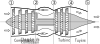
\includegraphics[width=0.8\linewidth]{thermo_turboreacteur.pdf}
\end{figure}

On formule les hypothèses suivantes pour les différentes transformations :
\begin{itemize}

	\item[$1\rightarrow2$ :] Compresseur, compression adiabatique réversible au taux de compression $a=P_2/P_1=26$ ;
	\item[$2\rightarrow3$ :] Chambre de combustion, le gaz est chauffé jusqu'à $T_3=1450$K de manière isobare ;
	\item[$3\rightarrow4$ :] Détente adiabatique réversible du gaz de $P_3$ et $P_4$ à travers la turbine ;
	\item[$5\rightarrow6$ :] Détente adiabatique réversible du gaz de $P_4$ et $P_5$ dans la tuyère.

\end{itemize}

On supposera que le régime est stationnaire, que l'énergie potentielle de pesanteur du fluide est négligeable dans toutes les étapes. L'énergie cinétique sera aussi négligée dans toutes les étapes, sauf à la sortie de la tuyère (en 5) où le gaz est très fortement accéléré. On négligera tout frottement mécanique. Les pressions en entrée et en sortie sont $P_1=P_5=1$ bar et la température en entrée est $T_1=288$K. On note $C_p$ la capacité thermique massique de l'air.

\begin{enumerate}

	\item En utilisant un bilan de masse et d'énergie, montrer que le travail massique utile reçu par le gaz lors d'une transformation de l'état $i$ à $j$ (sauf pour $2\rightarrow3$, dans la chambre de combustion) est donné par :
	\begin{align*}
		w_{i\rightarrow j}=C_p(T_j-T_i) + \frac{1}{2}\left(c_j^2-c_i^2 \right) 
	\end{align*}
	\item Donner une relation entre $P_i$, $P_j$, $T_i$, $T_j$ et $\gamma$ (sauf pour $2\rightarrow3$).
	\item En exploitant le couplage mécanique entre la turbine et le compresseur, établir les expressions littérales et les valeurs numériques des températures $T_2$, $T_4$ et de la pression $P_4$ en sortie de turbine.
	\item En déduire la vitesse $c_5$ à la sortie du réacteur. 
	\item \textit{(PSI, PC)} En déduire la poussée du réacteur en kN.

\end{enumerate}

\textit{Données :} $C_p=1,0\times10^3$J.kg$^{-1}$.K$^{-1}$, $\gamma=1,4$

\newpage

\section{Etude d'un turborécteur $\bullet\bullet\bullet\bullet$}

Un turboréacteur est un moteur thermique équipant les avions dits \textit{à réaction}, schématisé ci-dessous. Le fonctionnement général est le suivant : un turbine aspire et comprime l'air en amont du réacteur (étape $1\rightarrow2$), qui est ensuite chauffé par la combustion du kérosène dans la chambre de combustion (étape $2\rightarrow3$). Les gaz de combustion sont alors détendus ($3\rightarrow4$) à travers une turbine dont l'arbre est commun avec celui du compresseur, puis ces gaz sont finalement évacués par la tuyère ($4\rightarrow5$), en accélérant fortement, fournissant la poussée requise.

Le but de l'exercice est de calculer la vitesse de sortie $c_5$ des gaz de combustion, fournissant la poussée à l'aéronef.

\begin{figure}[!h]
\centering
	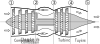
\includegraphics[width=0.8\linewidth]{thermo_turboreacteur.pdf}
\end{figure}

On formule les hypothèses suivantes pour les différentes transformations :
\begin{itemize}

	\item[$1\rightarrow2$ :] Compresseur, compression adiabatique réversible au taux de compression $a=P_2/P_1=26$ ;
	\item[$2\rightarrow3$ :] Chambre de combustion, le gaz est chauffé jusqu'à $T_3=1450$K de manière isobare ;
	\item[$3\rightarrow4$ :] Détente adiabatique réversible du gaz de $P_3$ et $P_4$ à travers la turbine ;
	\item[$5\rightarrow6$ :] Détente adiabatique réversible du gaz de $P_4$ et $P_5$ dans la tuyère.

\end{itemize}

On supposera que le régime est stationnaire, que l'énergie potentielle de pesanteur du fluide est négligeable dans toutes les étapes. L'énergie cinétique sera aussi négligée dans toutes les étapes, sauf à la sortie de la tuyère (en 5) où le gaz est très fortement accéléré. On négligera tout frottement mécanique. Les pressions en entrée et en sortie sont $P_1=P_5=1$ bar et la température en entrée est $T_1=288$K. On rappelle que la masse molaire de l'air est $M=29$g.mol$^{-1}$. 

\vspace{1cm}

Calculer la vitesse d'éjection $c_5$ des gaz à la sortie de la tuyère et en déduire la poussée que peut fournir ce turboréacteur.

\newpage

\begin{correction}

\begin{enumerate}

	\item Il s'agit simplementde la démonstration du premier principe industriel appliqué sur une transformation $i\rightarrow j$ (à demander dans la question).
	
	\item On utilise la loi de Laplace, valide pour toutes les transformations sauf lors de la combustion (l'hypothèse adiabatique n'est plus valide) :
	\begin{align*}
		P_1^{1-\gamma}T_1^\gamma&=P_2^{1-\gamma}T_2^\gamma \\
		P_3^{1-\gamma}T_3^\gamma&=P_4^{1-\gamma}T_4^\gamma \\
		P_4^{1-\gamma}T_4^\gamma&=P_5^{1-\gamma}T_5^\gamma \\
	\end{align*}
	
	\item Avec le rapport de compression $a$: 
	\begin{align*}
		T_2=&T_1a^{\frac{\gamma-1}{\gamma}} \\
		=&731K
	\end{align*}
	Ensuite, on utilise le couplage mécanique de l'arbre entre la turbine et le compresseur : $w_{1\rightarrow2}=C_p(T_2-T_1) =-w_{3\rightarrow}=C_p(T_4-T_3)$
	On a alors :
	\begin{align*}
		T_4=& T_3-(T_2-T_1)\\
		=& T_3-T_1\left(a^\frac{\gamma-1}{\gamma}-1 \right) \\
		=&907\mathrm{K}
	\end{align*}
	Pour la pression $P_4$, on utilise la transformation isobare dans la chambre de combustion :
	\begin{align*}
		P_4&=P_3\left(\frac{T_3}{T_4} \right)^\frac{\gamma}{1-\gamma}\\
		&=aP_1\left(\frac{T_3}{T_4} \right)^\frac{\gamma}{1-\gamma} \\
		&=6,5 \mathrm{bars}
	\end{align*}
	Et enfin pour $T_5$ :
	\begin{align*}
		T_5&=T_4\left(\frac{P_4}{P_5} \right) ^{\frac{\gamma-1}{\gamma}} \\
		&=T_3a^{\frac{1-\gamma}{\gamma}}\\
		&=532\mathrm{K}
	\end{align*}
	
	\item Avec le premier principe industriel, on a :
	\begin{align*}
		c_5=&\sqrt{2C_p(T_4-T_5)} \\
		=&866\mathrm{m.s}^{-1}
	\end{align*}
	
	
\end{enumerate}

\end{correction}